% XeLaTex
%\documentclass[review]{cvpr}
\documentclass[final]{cvpr}

\usepackage[UTF8]{ctex}

%\usepackage{cvpr}
\usepackage{times}
\usepackage{epsfig}
\usepackage{graphicx}
\usepackage{amsmath}
\usepackage{amssymb}
\usepackage{subfigure}
\usepackage{overpic}
\usepackage{color}
\usepackage{enumitem}
\setenumerate[1]{itemsep=0pt,partopsep=0pt,parsep=\parskip,topsep=5pt}
\setitemize[1]{itemsep=0pt,partopsep=0pt,parsep=\parskip,topsep=5pt}
\setdescription{itemsep=0pt,partopsep=0pt,parsep=\parskip,topsep=5pt}


\usepackage[pagebackref=true,breaklinks=true,colorlinks,bookmarks=false]{hyperref}


%\cvprfinalcopy % *** Uncomment this line for the final submission

\def\cvprPaperID{159} % *** Enter the CVPR Paper ID here
\def\confYear{CVPR 2020}
\def\httilde{\mbox{\tt\raisebox{-.5ex}{\symbol{126}}}}

\newcommand{\cmm}[1]{\textcolor[rgb]{0,0.6,0}{CMM: #1}}
\newcommand{\todo}[1]{{\textcolor{red}{\bf [#1]}}}
\newcommand{\alert}[1]{\textcolor[rgb]{.6,0,0}{#1}}

\newcommand{\IT}{IT\cite{98pami/Itti}}
\newcommand{\MZ}{MZ\cite{03ACMMM/Ma_Contrast-based}}
\newcommand{\GB}{GB\cite{conf/nips/HarelKP06}}
\newcommand{\SR}{SR\cite{07cvpr/hou_SpectralResidual}}
\newcommand{\FT}{FT\cite{09cvpr/Achanta_FTSaliency}}
\newcommand{\CA}{CA\cite{10cvpr/goferman_context}}
\newcommand{\LC}{LC\cite{06acmmm/ZhaiS_spatiotemporal}}
\newcommand{\AC}{AC\cite{08cvs/achanta_salient}}
\newcommand{\HC}{HC-maps }
\newcommand{\RC}{RC-maps }
\newcommand{\Lab}{$L^*a^*b^*$}
\newcommand{\mypara}[1]{\paragraph{#1.}}

\graphicspath{{figures/}}

% Pages are numbered in submission mode, and unnumbered in camera-ready
%\ifcvprfinal\pagestyle{empty}\fi
\setcounter{page}{1}

\begin{document}
% \begin{CJK*}{GBK}{song}

\renewcommand{\figref}[1]{图\ref{#1}}
\renewcommand{\tabref}[1]{表\ref{#1}}
\renewcommand{\equref}[1]{式\ref{#1}}
\renewcommand{\secref}[1]{第\ref{#1}节}
\def\abstract{\centerline{\large\bf 题目介绍} \vspace*{12pt} \it}

%%%%%%%%% TITLE

\title{机器学习第二次作业}

\author{朱一凡 \quad 计算机学院 \quad2120200467}

\maketitle
% \thispagestyle{empty}

%%%%%%%%% ABSTRACT
\begin{abstract}
    1.(20分)在讲稿第9页最下面的“注意”中指出:通过令两个偏导数为零,我们获得了最
    优参数值的必要条件,它们意味着预测误差是{\color{red}零均值}且{\color{red}与输入不相关}。
    试说明“零均值”和“不相关”的根据是什么?\par
    2.线性回归问题:假设存在直线方程$y=1.4x+0.9$,噪声服从分布$\mathcal{N}(0,5)$。\par
    \hspace{0.5cm}1)(10分)生成满足条件的100个独立同分布样本,选择其中$80\%$作为训练样本,剩
    余为测试样本。\par
    \hspace{0.5cm}2)(10分)绘出训练样本和测试样本的散布图。\par
    \hspace{0.5cm}3)(30分)编程实现求解线性回归的最小二乘法和采用Huber损失函数的鲁棒线性回
    归方法。\par
    \hspace{0.5cm}4)(10分)使用3)中实现的线性回归方法求解训练样本的线性回归方程,并给出测试
    样本的均方误差。\par
    \hspace{0.5cm}5)(20分)解释4)中你所得到的结果,并对两种求解方法进行比较。
\end{abstract}




%%%%%%%%% BODY TEXT %%%%%%%%%%%%%%%%%%%%%%%%%%%%%%%%%%%%%%%%
\section{第一题}\label{sec:Introduction}
\subsection{问题描述}
通过两个偏导数为$0$这一条件推导出此时预测误差是 {\color{red}零均值}且{\color{red}与输入不相关}这一结论。问题难点在于构建出
偏导数为$0$和结论之间连接的桥梁。
\subsection{基本思路}
输入误差是零均值意味着有下列式子的成立,其中y为观测输出,x为输入,$\mathbf{w}$为估计的权值。
\begin{equation}
    E(y_i-w_0-w_1x_i)=\sum_{i=0}^n y_i-w_0-w_1x_i=0
\label{eq1}
\end{equation}
与输入不相关意味着对于任意输入,结论是不变化的。\par
为了得到上述结论,可以将导数为0时的式子进行变形。
\subsection{解题步骤}
当两个导数都为0时,有以下式子成立:
\begin{equation}
    \frac{\partial}{\partial w_{0}} J_{N}(\mathbf{w})=-\sum_{i=1}^{N}\left(y_{i}-w_{0}-w_{1} x_{i}\right)=0 
\label{eq2}
\end{equation}
\begin{equation}
    \frac{\partial}{\partial w_{1}} J_{N}(\mathbf{w})=-\sum_{i=1}^{N}\left(y_{i}-w_{0}-w_{1} x_{i}\right) x_{i}=0
\label{eq3}
\end{equation}
当式\ref{eq2}成立时,有$\sum_{i=0}^n(y_i-w_0-w_1x_i)=0$,所以预测误差的均值为0。对于式\ref{eq3},有
$(\sum_{i=0}^n(y_i-w_0-w_1x_i))(\sum_{i=0}^nx_i)=0$,故其与输入$x_i$不相关
%%%%%%%%%%%%%%%%%%%%%%%%%%%%%%%%%%%%%%%%%%%%%%%%%%%%%%%%%%%%%%%%%%%%%%
\section{第二题}\label{sec:Experiment}
\subsection{问题描述}
该问题是一个线性回归问题,需要自己完成数据的生成和对两种回归算法的比较分析。难点在于编程实现时的算法细节处理。
\subsection{基本思路}
首先使用随机数和采样实现算法的数据的生成。在生成数据的时候,首先生成x,在实验中使用 $x \in [-10,10]$ ,均匀的在$x$的区间进行采样。
然后根据公式$y = 1.4x+0.9 + \mathcal{N}(0,5)$来得到$y$的值。随机误差可使用numpy所自带的库来生成。\par
在得到数据后,编程实现两种回归方法。最小二乘回归比较简单,可以直接使用表达式得到最终的结果。Huber损失函数的鲁棒线性回归方法则需要使用梯度下降法
来进行求解。梯度下降法可以使用pytorch进行实现。
\subsection{解题步骤}
\subsubsection{处理流程}
首先进行数据的生成。在算法中使用均匀采样的方法在$[-10,10]$区间上采样100次得到$x$,随后使用公式$y = 1.4x+0.9 + \mathcal{N}(0,5)$
来得到$y$的值。在得到全部的数据之后,使用随机抽样的方法来确定训练集和测试集。每一次的数据使用一个类函数来表达。绘制散点图可以使用Python中的matplotlib库
进行实现。\par
在得到训练数据和测试数据之后,可以进行回归算法的实现。实现两种回归算法,分别计算这两种算法在测试集上的均方误差。详细的计算过程在算法描述部分进行讨论。
\subsubsection{算法描述}
首先进行数据的生成。在算法中使用均匀采样的方法在$[-10,10]$区间上采样100次得到$x$,随后使用公式$y = 1.4x+0.9 + \mathcal{N}(0,5)$
来得到$y$的值。在得到全部的数据之后,使用随机抽样的方法来确定训练集和测试集。每一次的数据使用一个类函数来表达。绘制散点图可以使用Python中的matplotlib库
进行实现。由于随机数的生成具有不确定性,所以进行多次生成以确保算法的有效性。\par
在得到训练数据和测试数据之后,可以进行回归算法的实现。对于最小二乘法来说,在处理线性回归时,可以使用以下的公式进行计算
\begin{equation}
    \hat{w} = (X^TX)^{-1}X^Ty
\end{equation}
均方误差可以使用以下公式进行计算
\begin{equation}
    MSE = \sum_{i=0}^{n}{(y-\hat{y})^2}
\end{equation}
对于Huber损失函数的鲁棒线性回归方法,使用Huber损失函数作为最终的优化目标。其形式如下:
\begin{equation}
    L_{H u b e r}(r, \delta)=\left\{\begin{array}{cl}
        r^{2} / 2 & \text { if }|r| \leq \delta \\
        \delta|r|-\delta^{2} / 2 & \text { otherwise }
        \end{array}\right.
\end{equation}
随后使用梯度下降法进行求解。梯度下降法使用pytorch实现,在算法中仅这一部分借助库函数实现。
\subsubsection{算法实现(Python语言源代码)}
算法的实现结果如附件中的代码所示。使用Python语言实现,主要使用了numpy,matplotlib,pytorch算法库。
\subsection{结果与分析}
\subsubsection{实验内容与步骤}
实验内容主要由三部分构成,数据的生成,最小二乘算法回归分析,Huber损失函数法回归分析。首先将数据的范围
固定到$[-10,10]$,生成100组实验数据进行图像的绘制和回归分析。随后改变数据的取值范围,观察其对算法
的影响。其中Huber的参数为0.1,最大训练200次。
\subsubsection{实验结果}
首先将数据的范围固定到$[-10,10]$,生成100组实验数据进行图像的绘制和回归分析.结果如图\ref{fig1}\par
\begin{figure}[htbp]
    \centering
    \subfigure[数据分布]{
    \begin{minipage}[t]{0.33\linewidth}
    \centering
    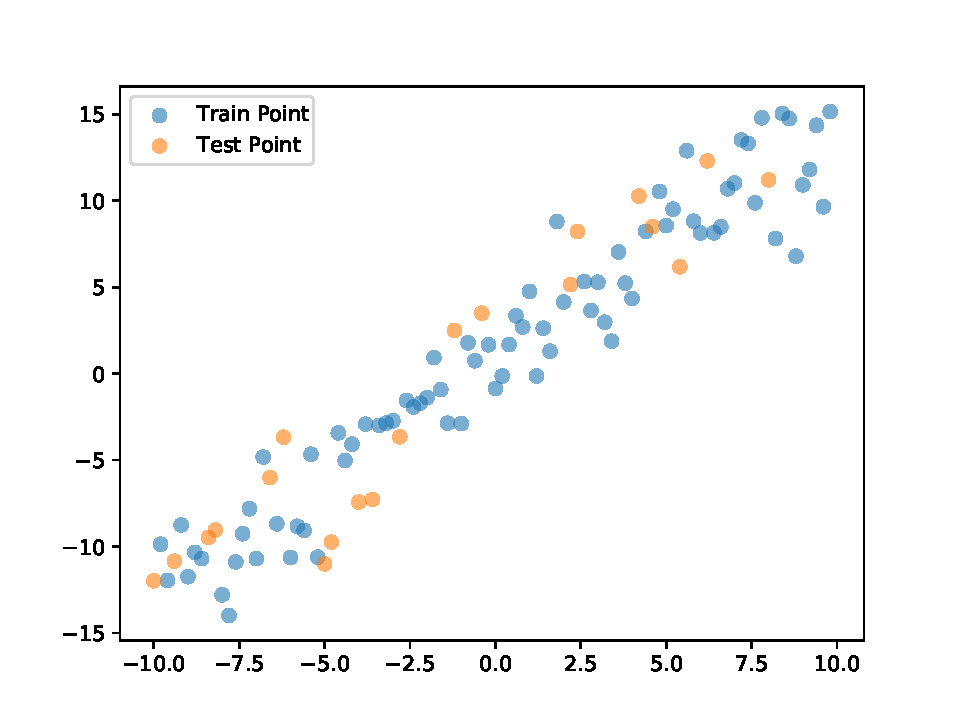
\includegraphics[width=2.5in]{figures/data1.pdf}
    %\caption{fig1}
    \end{minipage}%
    }%
    \subfigure[最小二乘法结果]{
    \begin{minipage}[t]{0.33\linewidth}
    \centering
    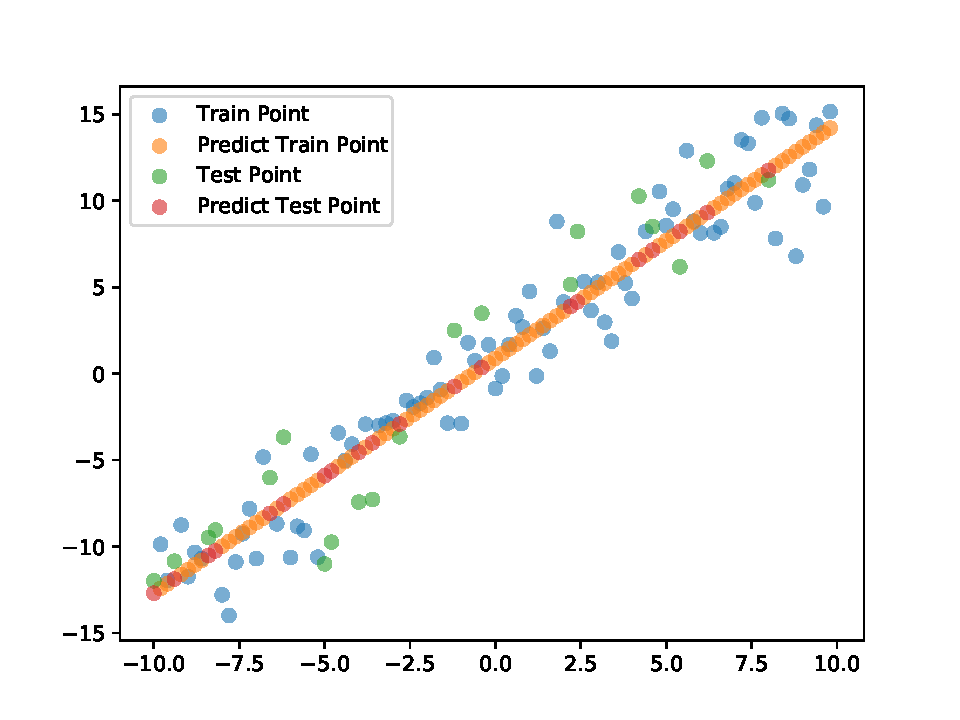
\includegraphics[width=2.5in]{figures/zuixiao.pdf}
    %\caption{fig2}
    \end{minipage}%
    }%                    %这个回车键很重要 \quad也可以
    \subfigure[Huber损失函数法结果]{
    \begin{minipage}[t]{0.33\linewidth}
    \centering
    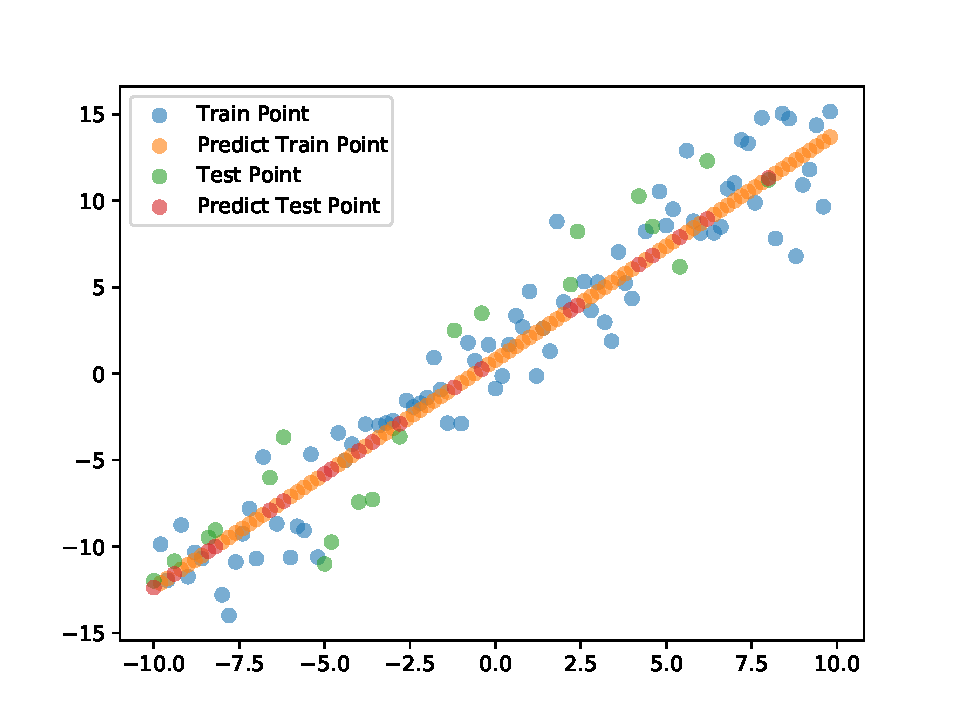
\includegraphics[width=2.5in]{figures/huber1.pdf}
    %\caption{fig2}
    \end{minipage}
    }%
    \centering
    \caption{$x \in [-10,10]$}
    \label{fig1}
    \end{figure}
最终结果:\par
最小二乘法:$y = 1.35x+0.88$, $MSE = 7.94$\par
Huber法损失函数:$y = 1.37x+0.89$, $MSE = 7.65 $
将数据的范围固定到$[-1,1]$,生成100组实验数据进行图像的绘制和回归分析.结果如图\ref{fig2}\par
\begin{figure}[htbp]
    \centering
    \subfigure[数据分布]{
    \begin{minipage}[t]{0.33\linewidth}
    \centering
    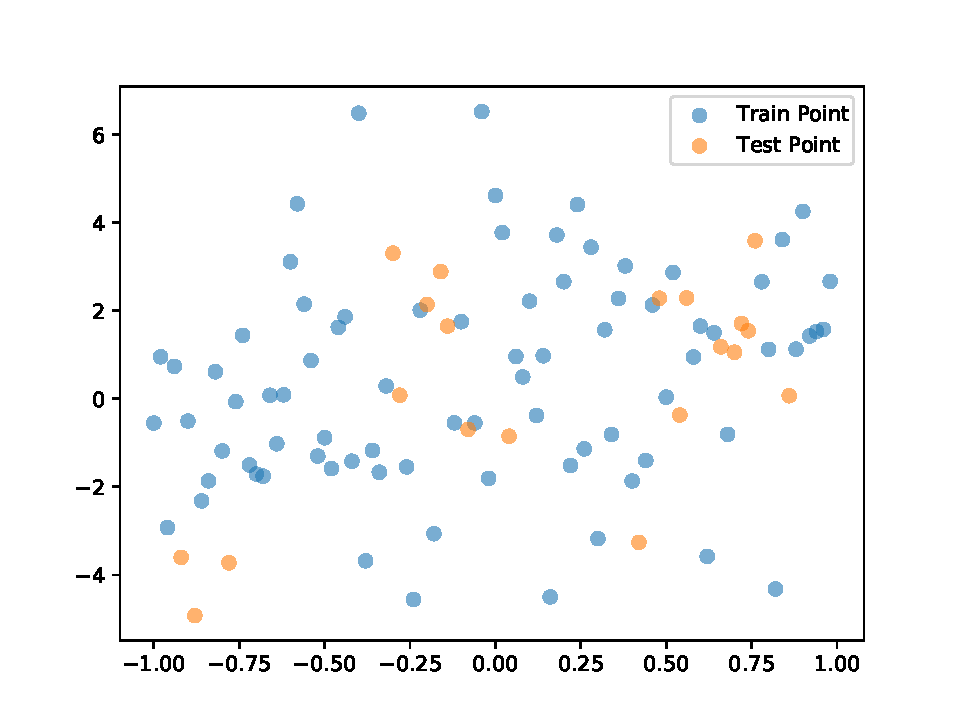
\includegraphics[width=2.5in]{figures/data2.pdf}
    %\caption{fig1}
    \end{minipage}%
    }%
    \subfigure[最小二乘法结果]{
    \begin{minipage}[t]{0.33\linewidth}
    \centering
    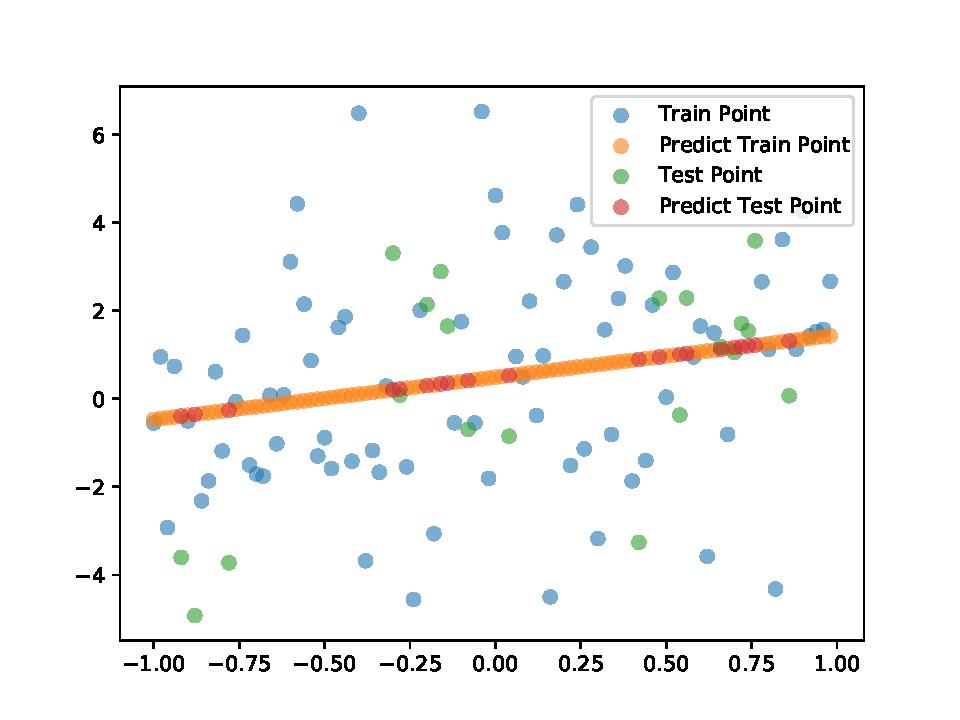
\includegraphics[width=2.5in]{figures/zuixiao2.pdf}
    %\caption{fig2}
    \end{minipage}%
    }%                    %这个回车键很重要 \quad也可以
    \subfigure[Huber损失函数法结果]{
    \begin{minipage}[t]{0.33\linewidth}
    \centering
    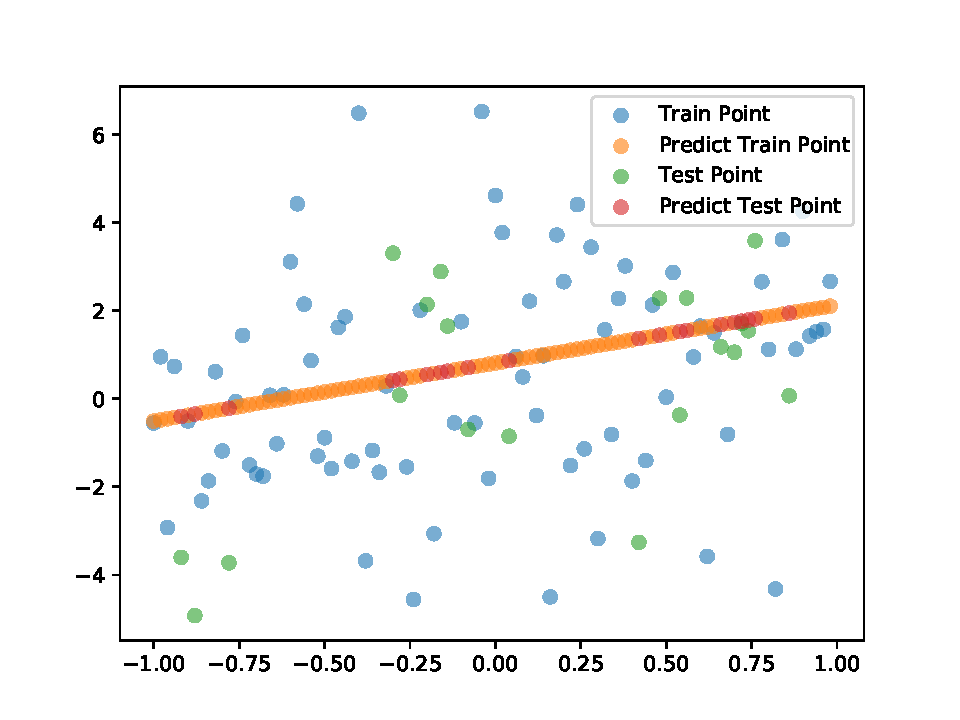
\includegraphics[width=2.5in]{figures/huber2.pdf}
    %\caption{fig2}
    \end{minipage}
    }%
    \centering
    \caption{$x \in [-1,1]$}
    \label{fig2}
    \end{figure}
最终结果:\par
最小二乘法:$y = 0.95x+0.48$, $MSE = 5.97 $\par
Huber法损失函数:$y = 1.31x+0.81$, $MSE = 4.88 $
将数据的范围固定到$[-100,100]$,生成100组实验数据进行图像的绘制和回归分析.结果如图\ref{fig3}\par
\begin{figure}[htbp]
    \centering
    \subfigure[数据分布]{
    \begin{minipage}[t]{0.33\linewidth}
    \centering
    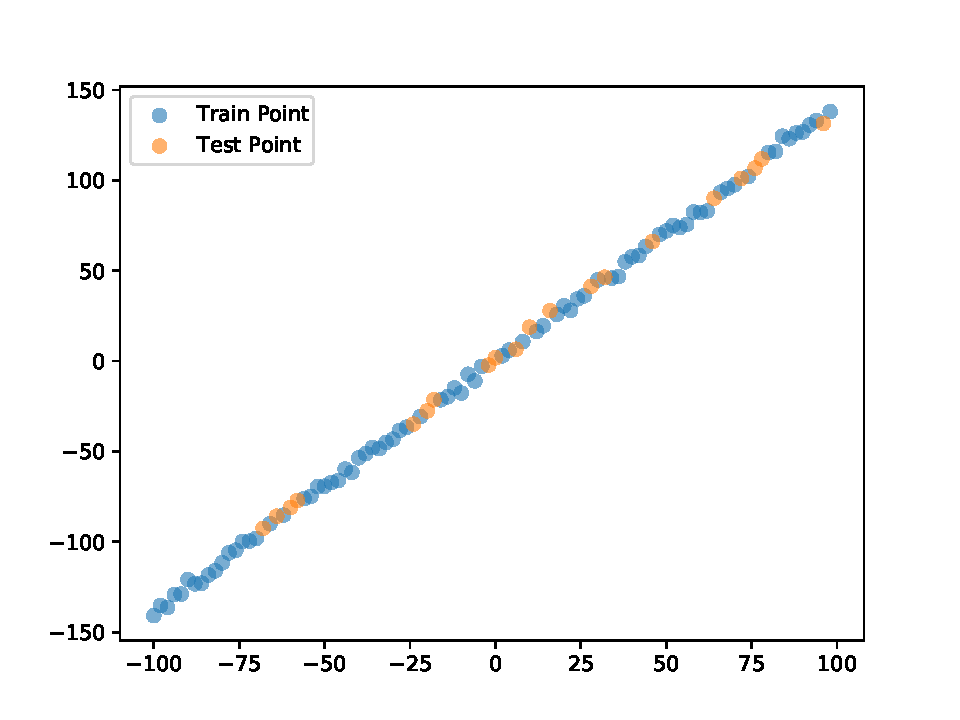
\includegraphics[width=2.5in]{figures/data3.pdf}
    %\caption{fig1}
    \end{minipage}%
    }%
    \subfigure[最小二乘法结果]{
    \begin{minipage}[t]{0.33\linewidth}
    \centering
    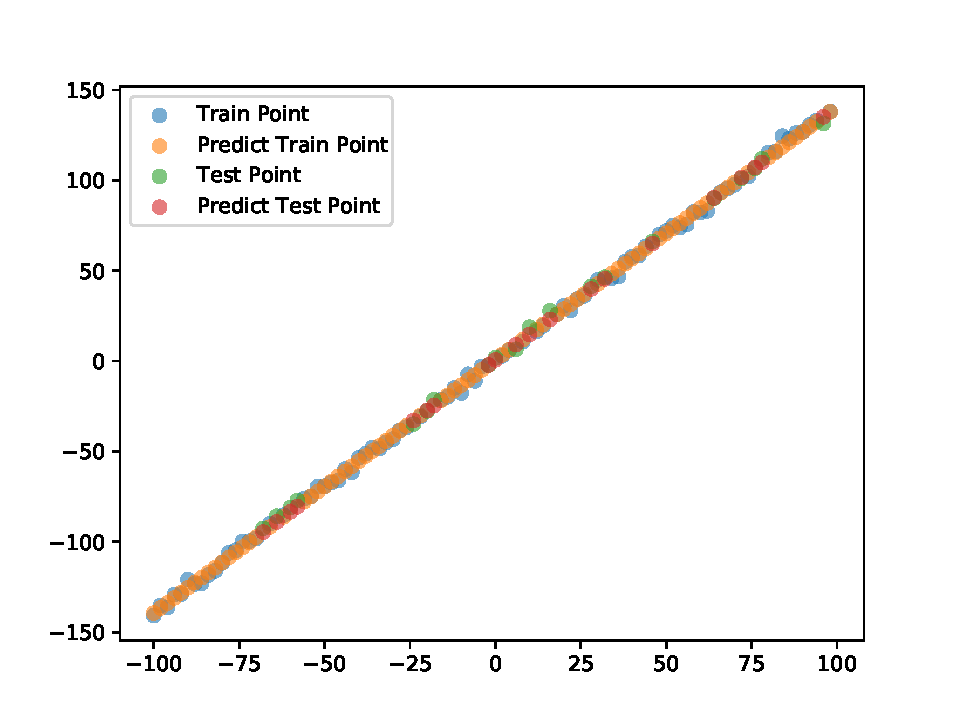
\includegraphics[width=2.5in]{figures/zuixiao3.pdf}
    %\caption{fig2}
    \end{minipage}%
    }%                    %这个回车键很重要 \quad也可以
    \subfigure[Huber损失函数法结果]{
    \begin{minipage}[t]{0.33\linewidth}
    \centering
    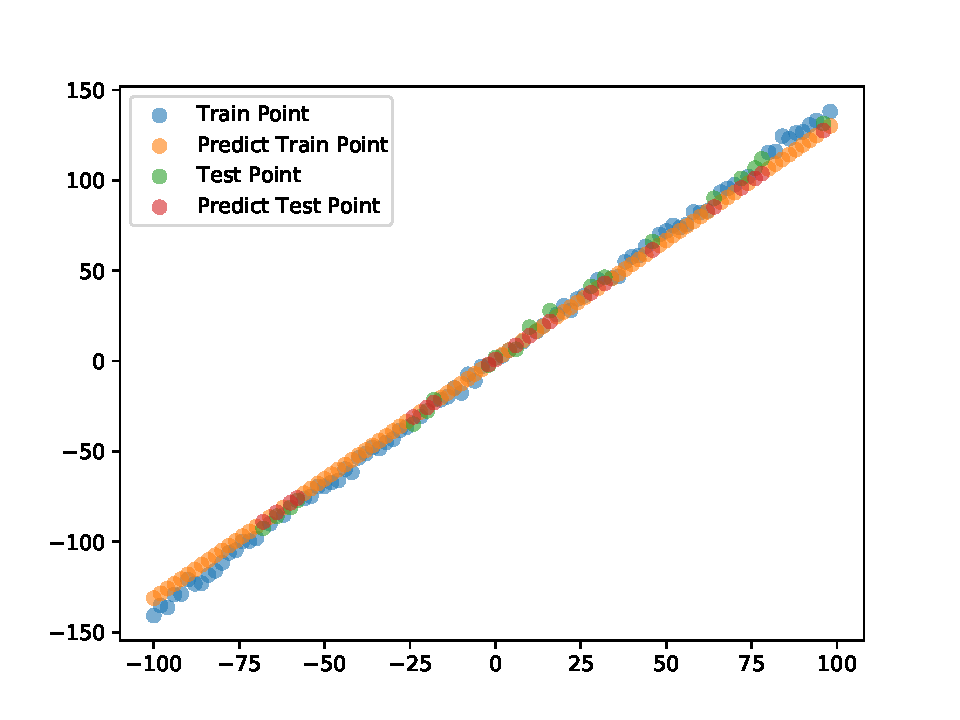
\includegraphics[width=2.5in]{figures/huber3.pdf}
    %\caption{fig2}
    \end{minipage}
    }%
    \centering
    \caption{$x \in [-100,100]$}
    \label{fig3}
    \end{figure}
最终结果:\par
最小二乘法:$y = 1.40x+0.65$, $MSE = 5.74 $\par
Huber法损失函数:$y = 1.38x+0.78$, $MSE = 7.88 $
\subsubsection{结果分析}
可以看到,在上述的结果中,前两种情形Huber方法的均方差都要比最小二乘法要小。这是因为Huber损失函数可以很好地减少误差比较大的点
对于回归结果的影响。但是最小二乘法却无法做到。但是最小二乘法的计算相比于Huber损失函数要更容易计算。在生成数据的区间比较小的时候,生成的数据更难
进行回归处理。这是因为当数据范围比较小的时候收到误差的影响要更大,所以更难进行处理。而此时的Huber方法相对于最小二乘法的提高也是最大的。但是当数据范围变大时,由于
误差点的影响很小,所以此时的最小二乘法有了更好的表现。当然,Huber的参数也会影响到算法的性能,在此不做讨论。此外,当范围不同的时候,均方误差会因为y的值域不同而有所不同。
%%%%%%%%%%%%%%%%%%%%%%%%%%%%%%%%%%%%%%%%%%%%%%%%%

\section{总结}\label{sec:Conclusion}
在这次实验中我体会到了数据分布对于一个算法的成功与否十分的重要。在生成数据范围比较小的时候,很难学习到一个正确
的结果。当数据的范围扩大时,才能得到一个比较准确的结果。并且Huber损失函数法要比最小二乘法更好地适应离群点对
算法的影响,相比于最小二乘法更加稳定。但是不同的算法有不同的使用情况,一定要慎重选择。





% \end{CJK*}
\end{document}
